\documentclass[10pt,a4paper]{article}
\usepackage[margin=18mm]{geometry}
\usepackage[T1]{fontenc}
\usepackage{lmodern,graphicx,booktabs,amsmath,amssymb,array}
\usepackage[hidelinks]{hyperref}
\setlength{\parindent}{0pt}
\setlength{\parskip}{5pt}
\begin{document}
{\Large\bfseries An actual genus-two realization of the chained pair Prym}\par
{\large\bfseries Two explicit covers and a global retraction of the beta3 image}\par
24 November 2026 \quad crypto PR5114 \quad [pcc:unverified]

\textbf{Concrete result.} The primitive degree-four cover from the actual
CM19 plane quartic produces an $S_4$ pair resolvent with an etale double
cover $Y_6\to Y_3$, of genera five and three. Its principally polarized
Prym is now identified with the Jacobian of an explicit genus-two curve
over the original prime field. The actual chained map $\Gamma_D:E\to J(D)$
has a global left inverse, not only an inverse on odd-order points.
\[
\begin{gathered}
E/\mathbb F_7:\quad v^2=u^3+2u+6,\qquad \#E(\mathbb F_7)=11,\quad T=(1,3),\\
D/\mathbb F_7:\quad Y^2=6W^6+2W^4+1,\\
p_1:D\to E,\quad (W,Y)\mapsto(3W^2+5,Y),\qquad
p_2:D\to E,\quad (W,Y)\mapsto(W^{-2},YW^{-3}),\\
\boxed{\ p_{1*}\Gamma_D=I,\qquad p_{2*}\Gamma_D=\bar\omega\ },
\qquad \omega=\pi+2,\quad\omega^2-\omega+5=0.
\end{gathered}
\]
The boxed identities are written actual-Jacobian deductions in claim
8b16d2, following native D a6653a and geometric proof d80057. Full
Mumford arithmetic is the next implementation; the current program does
not claim to execute the entire Jacobian chain. All claims are unsigned.

\begin{center}
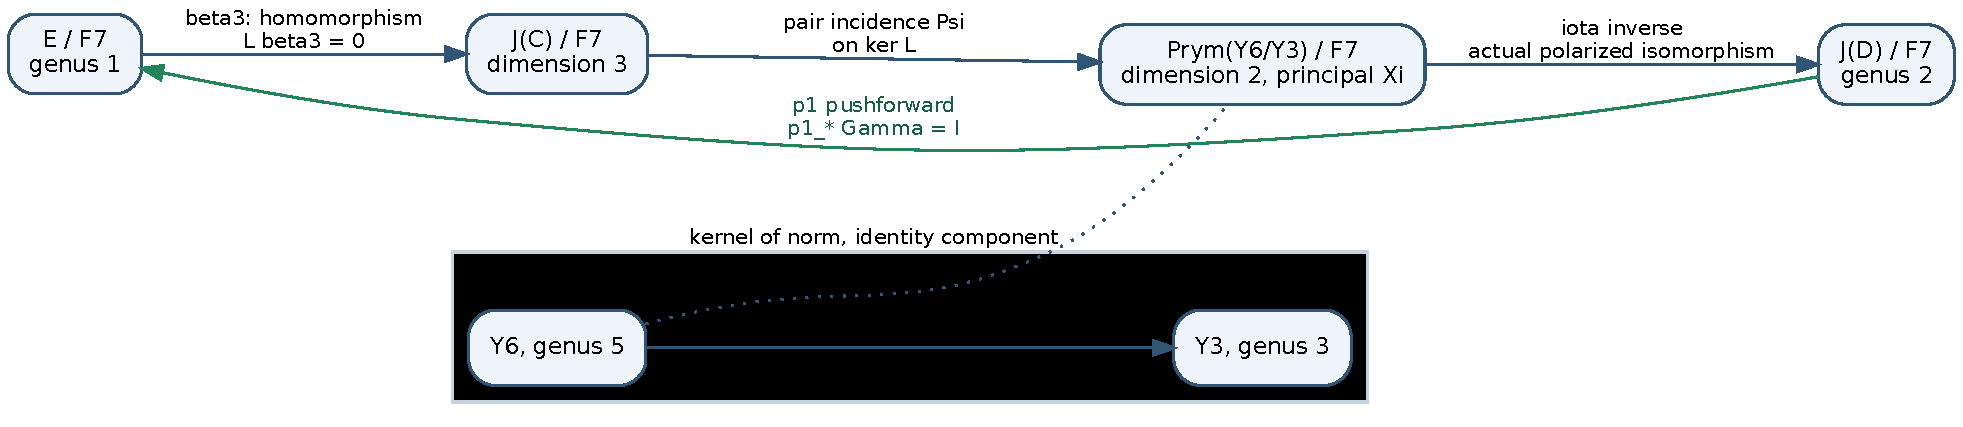
\includegraphics[width=\linewidth,height=72mm,keepaspectratio]{chain.pdf}
\end{center}
\textbf{Why this is the actual Prym.} Let $K=\ker L\subset J(C)$, with
actual basis $a=\beta(1,-\omega,0)$ and $b=\beta_3$. The incidence
map $j:K\to P$ has degree four and principal pullback
\[
G=\begin{pmatrix}16&-4-2\omega\\-6+2\omega&3\end{pmatrix},\quad
\det G=4,\qquad \ker j=a(E[2]).
\]
Consequently $ja$ is genuinely divisible by two in the integral Hom
group. In the resulting principal basis $(c,d)$, with $d=jb$, one obtains
\[
H_P=\begin{pmatrix}2&\bar\omega\\\omega&3\end{pmatrix},\quad
e=-\bar\omega c+2d,\quad S=(e,c),\quad S^\dagger H_P S=2I.
\]
The ordered kernel of $S$ is $\{(Q,\bar\omega Q):Q\in E[2]\}$.
On actual two-torsion, $\bar\omega=\pi^2$ is Frobenius49. The two covers
give $\Omega=(p_1^*,p_2^*)$ with the same ordered graph kernel and
polarization $2I$. The quotient property yields an actual polarized
$\iota:J(D)\simeq P$, with $\iota\Omega=S$; a matching Weil polynomial
alone would not establish this identification.

\textbf{Primary theorem boundary.} Beauville, Inventiones 41 (1977),
Theorem 3.7/Lemma 3.8, provides the odd-characteristic Prym restriction
$\lambda_{J(Y_6)}|_P=2\Xi$. Howe--Leprevost--Poonen (2000),
Propositions 3/4 and Corollary 6, supplies the two-gluing quotient
framework. Here $j(E)=1\ne0,1728=6$, and Frobenius49 is a nonidentity,
Galois-equivariant two-torsion automorphism, distinct from restrictions
of $\operatorname{Aut}(E)=\{\pm1\}$. These are applications of established
theory to the actual objects; no novelty of those methods is claimed.

\newpage
{\Large\bfseries Exact certificates, geometry and preserved controls}\par

\textbf{The model is derived from the actual graph.} In
$\mathbb F_{343}=\mathbb F_7[\alpha]/(\alpha^3+2\alpha+6)$, all three
two-torsion roots and their Frobenius actions are explicit. The rank-three
Mobius system gives $M(x)=1/(5x+3)$ and $M(\alpha)=\alpha^{49}$.
The complete cubic identity is
\[
1+2(5x+3)^2+6(5x+3)^3=x^3+2x+6.
\]
The resulting sextic is squarefree, with a complete Bezout witness:
\[
(1+W^4)H+(4W+4W^3+W^5)H'=1,\quad
H=6W^6+2W^4+1,\quad H'=W^5+W^3.
\]
Both displayed covers satisfy full polynomial identities. At $W=0$,
$p_2$ extends to $O$ with pole orders two and three. At the two conjugate
infinity branches, $\eta^2=6$, $p_1$ extends to $O$ and $p_2$ to
$(0,\eta)$. There is no rational infinity point. All eight base fibres
are retained: fourteen finite rational points in total. Three actual
Weierstrass packets have $u=W^2-(5\alpha_i+3),v=0$ and give the shared
ordered graph. With $D_0=p_2^*O$, $D_\infty=p_1^*O$,
$\operatorname{div}(W)=D_0-D_\infty$. Proper extension and these divisor
identities, rather than a rational-point census, establish the maps.

\textbf{Integral retraction.} The actual quotient construction gives
\[
2\Gamma_D=p_1^*+p_2^*\bar\omega.
\]
Cross push--pull is zero, while $p_{i*}p_i^*=[2]$. Cancellation of
two in torsion-free $\operatorname{Hom}(E,E)$ proves the two global
identities on page one. Thus $\Gamma_D$ preserves every subgroup scheme.
On $E(\mathbb F_7)[11]$, $\omega$ acts as three, so an executable input
recipe is $\Gamma_D(P)=[6](p_1^*P+p_2^*[-2]P)$. Global existence comes
from the quotient argument; inverse two modulo eleven alone does not
construct a global map. Its principal norm is three. The earlier input
of norm124/ambient248 is retained; beta3 has input norm3/ambient6.

\begin{center}\small
\begin{tabular}{llllll}
\toprule
Unit & Source & Locked inputs & Phases & Full stdout & Data claim\\
\midrule
A primitive quartic & ec5226f2 & 33+lock & 7 pass & 50618 B & 11a40a\\
B actual incidence & cac861f9 & 60+lock & 7 pass & 18820 B & 7dafac\\
C split kernel & 7c33fc4e & 75+lock & 7 pass & 1905 B & 3de67e\\
D actual genus two & f8bb6fe8 & 101+lock & 7 pass & 6250 B & a6653a\\
\bottomrule
\end{tabular}\end{center}
Every input was published and read back whole before the first strict
call. Each unit uses pinned Rust1.99.1, warnings as errors, opt3,
overflow/debug assertions, one worker and 120 seconds/2 GiB per phase;
pre/post source, tool, runtime and executable-qualifier guards agree.
Each retains 38 whole small originals. Executed ELFs and separate0555
qualifiers of 4673800/4852096/4601288/4652960 bytes remain whole in RAM
pending approved custody; new CI artifacts are distinct originals.

\textbf{Negative controls and failures.} Real quartic, resolvent,
incidence and CM coefficient mutations reject and restore. C's changed
input keeps norm three but leaves $\ker L$; this result is retained.
D's changed gluing coefficient fails the full polarization identity;
changed sextic constant fails both cover identities. The initial
unlabeled graph direction was corrected in separate claim ff1474 before
D code. Natural sign and cubic correspondences factor the common
elliptic base, a scoped negative. No failed mathematical case is removed.

\textbf{Formal and signer boundary.} Crypto-lean38 contains two separately
frozen generic laws over genuine additive homomorphisms. Both first
attempts fail reading distinct existing Lean private-import files before
theorem checking; zero theorems are accepted and the canonical axiom audit
is not reached. No cap, auditor or keyring change is used. The geometric
proofs here remain written, and independent signed verification is open.

\newpage
{\Large\bfseries Scoped solver assessment and the next executable obligation}\par

\textbf{Exact diagnostic scope.} This is fixed mathematical correctness
over $\mathbb F_7$, with $T=(1,3)$, prime order11 and cofactor one.
The actual destination has order121 and rational group $C_{11}^2$ via
the prime-to-eleven $E^2$ isogeny. The image is the specified embedded
order-eleven subgroup. Extension fields343 (two-torsion) and49
(infinity branches) qualify geometry; the transfer is defined over the
same prime field. No proper prime-subfield descent occurs. There is no
timed workload, target batch, new registered curve/candidate or IC
leaderboard result; diagnostic work is excluded from those dashboards.

\textbf{Named solver and recovery interfaces.} Shanks baby-step giant-step
and Pollard rho apply to the transported cyclic subgroup once its group
operations are implemented. They receive $\Gamma_D(T)$ and
$\Gamma_D(Q)$ without the unknown scalar. A returned scalar is reused
unchanged modulo11 and must satisfy $[x]T=Q$. The structured cover route
first computes $p_{1*}$, yielding the original elliptic points. This
projection itself returns no unknown logarithm; its use as a standalone
solver is refuted. Existing elliptic solvers remain required. A cyclic
full-Jacobian index-calculus hypothesis cannot be assumed for $C_{11}^2$.

\begin{center}\small
\begin{tabular}{p{39mm}p{35mm}p{35mm}p{35mm}}
\toprule
Cold one-target phase & Direct source reference & Same generic solver on image & Covers plus source solver\\
\midrule
Search/prior selection & unpriced & unpriced & unpriced\\
Construction & unpriced & unpriced & unpriced\\
Map/input conversion & not applicable & unpriced & unpriced\\
Preprocessing & unpriced & unpriced & unpriced\\
Relations/collision search & unpriced & unpriced & unpriced\\
Linear algebra & not applicable & not applicable & not applicable\\
Individual log & unpriced & unpriced & unpriced\\
Recovery/conversion & unpriced & unpriced & unpriced\\
Source verification & unpriced & unpriced & unpriced\\
\bottomrule
\end{tabular}\end{center}
The source reference must include the strongest applicable automorphism
and parallel-rho configuration. Collision work belongs to the chosen
generic solver; it is never charged twice as both search and individual
log. Every applicable unpriced phase is unknown, not zero. No total,
net ratio, amortization, modeled advantage or measured advantage is
supported. Benchmarks or parameter searches retain the original
checkpoint, storage, EKS ownership and paid-admission requirements.

\begin{center}\small
\begin{tabular}{p{57mm}p{24mm}p{71mm}}
\toprule
Obligation & State & Evidence and scope\\
\midrule
Actual curve/covers/polarized bridge & supported & a6653a native; d80057 written geometry\\
Global homomorphism/preservation & supported & 8b16d2 written global left inverse\\
Scalar answer recovery & supported & identity scalar recovery from global left inverse\\
Executable source replay & unknown & full arithmetic interface pending\\
Complete executable divisor transfer & unknown & actual Mumford group implementation next\\
Named generic solver applicability & supported & cyclic order11 image; software interface pending\\
Projection alone solves unknown log & refuted & p1 pushforward returns original elliptic point\\
End-to-end modeled/measured cost & unknown & no priced three-arm experiment\\
Novel reduction/full formal theorem & unknown & established gluing; no clearance or accepted proof\\
\bottomrule
\end{tabular}\end{center}

\textbf{Next checkable component.} Prove the canonical degree-two
representation relative to conjugate infinity, enumerate all valid actual
Mumford ideals, implement Cantor composition/reduction, and compare the
complete group table with independently evaluated cover pushforwards.
Then check all eleven transferred inputs and an unknown-log interface
with source replay. Preserve complete tables and first failures. This
separate cryptanalysis component continues while feature-stack CI and
merge requirements remain pending. Full locks, proof maps, primary-source
links and original inventories live beside this report. [pcc:unverified]
\end{document}
